\section{Zavaró jel PI szabályozóval (Szorgalmi feladat)}\label{sec:szorg-pi}

Mivel a rendszerünk lineáris, ezért a két bemenetet kezelhetjük függetlenül.

Legyen a referencia feszültség bemenet Laplace-transzformáltja
$\mathrm{U}_\omega = \frac{\omega_\text{n}}{2s}$,
a zavarójel pedig legyen egy $\tau_0$ nagyságú ugrásfüggvény időben eltolva $T_0$-al,
ami elvileg végtelen: $\mathrm{U}_\tau=\frac{\tau_0}{s}\text{e}^{-T_0s}$.

A rendszer szögsebesség válasza ezekre a bemenetekre kiszámítható a hatásvázlat segítségével.

\begin{equation}
	\fn{Y} = \fn{W}_\text{p}\fn{U}_\text{p} + \fn{W}_{\text{p}\tau}\fn{U}_\tau
\end{equation}
\begin{equation}
	\fn{U}_\text{p} = \fn{W}_\text{c}\brc{\fn{U}_0 - \fn{Y}}
\end{equation}
\begin{equation}
	\fn{Y} = \frac{\fn{W}_\text{p}\fn{W}_\text{c}\fn{U}_0 + \fn{W}_{\text{p}\tau}\fn{U}_\tau}{\fn{W}_\text{p}\fn{W}_\text{c} +1}
\end{equation}
\begin{equation}
	\fn{y} = \mathcal{L}^{-1}\{\fn{Y}\}
\end{equation}

A szögsebességből az áram az alábbiak szerint számolható:
\begin{equation}
	\fn{i}_\text{a}(s) = \ke\fn{W}_\text{el}\brc{\fn{U}_0 - \fn{Y}_\omega}
\end{equation}

Ezeknek az egyenleteknek a behelyettesített változatát nem írom ki, mert
nagyon hosszú és csúnya, de a MATLAB kódban megtalálható.

\begin{figure}[H]
	\centering
	\begin{subfigure}{.49\textwidth}
		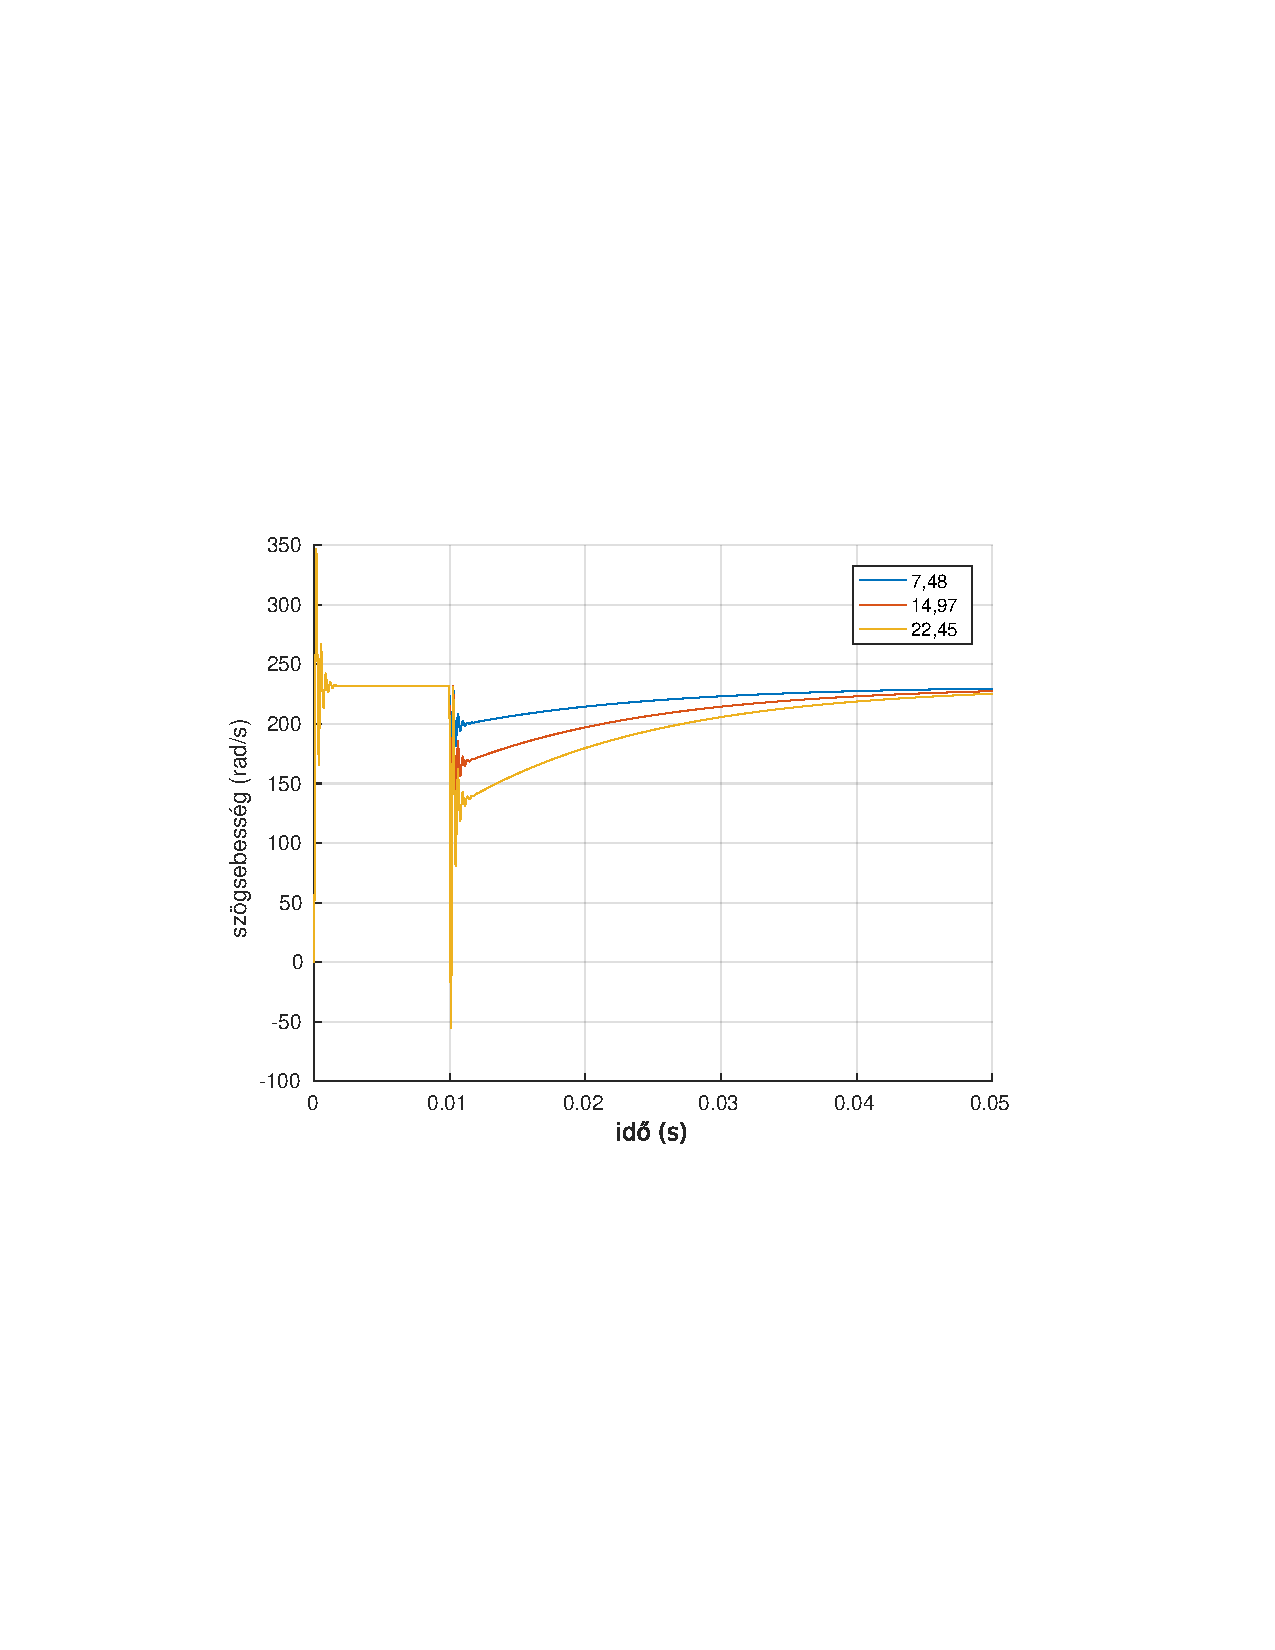
\includegraphics[width=\linewidth, trim=100 240 80 252, clip]{5-w}
		\caption{Szögsebesség válasz}
	\end{subfigure}
	\begin{subfigure}{.49\textwidth}
		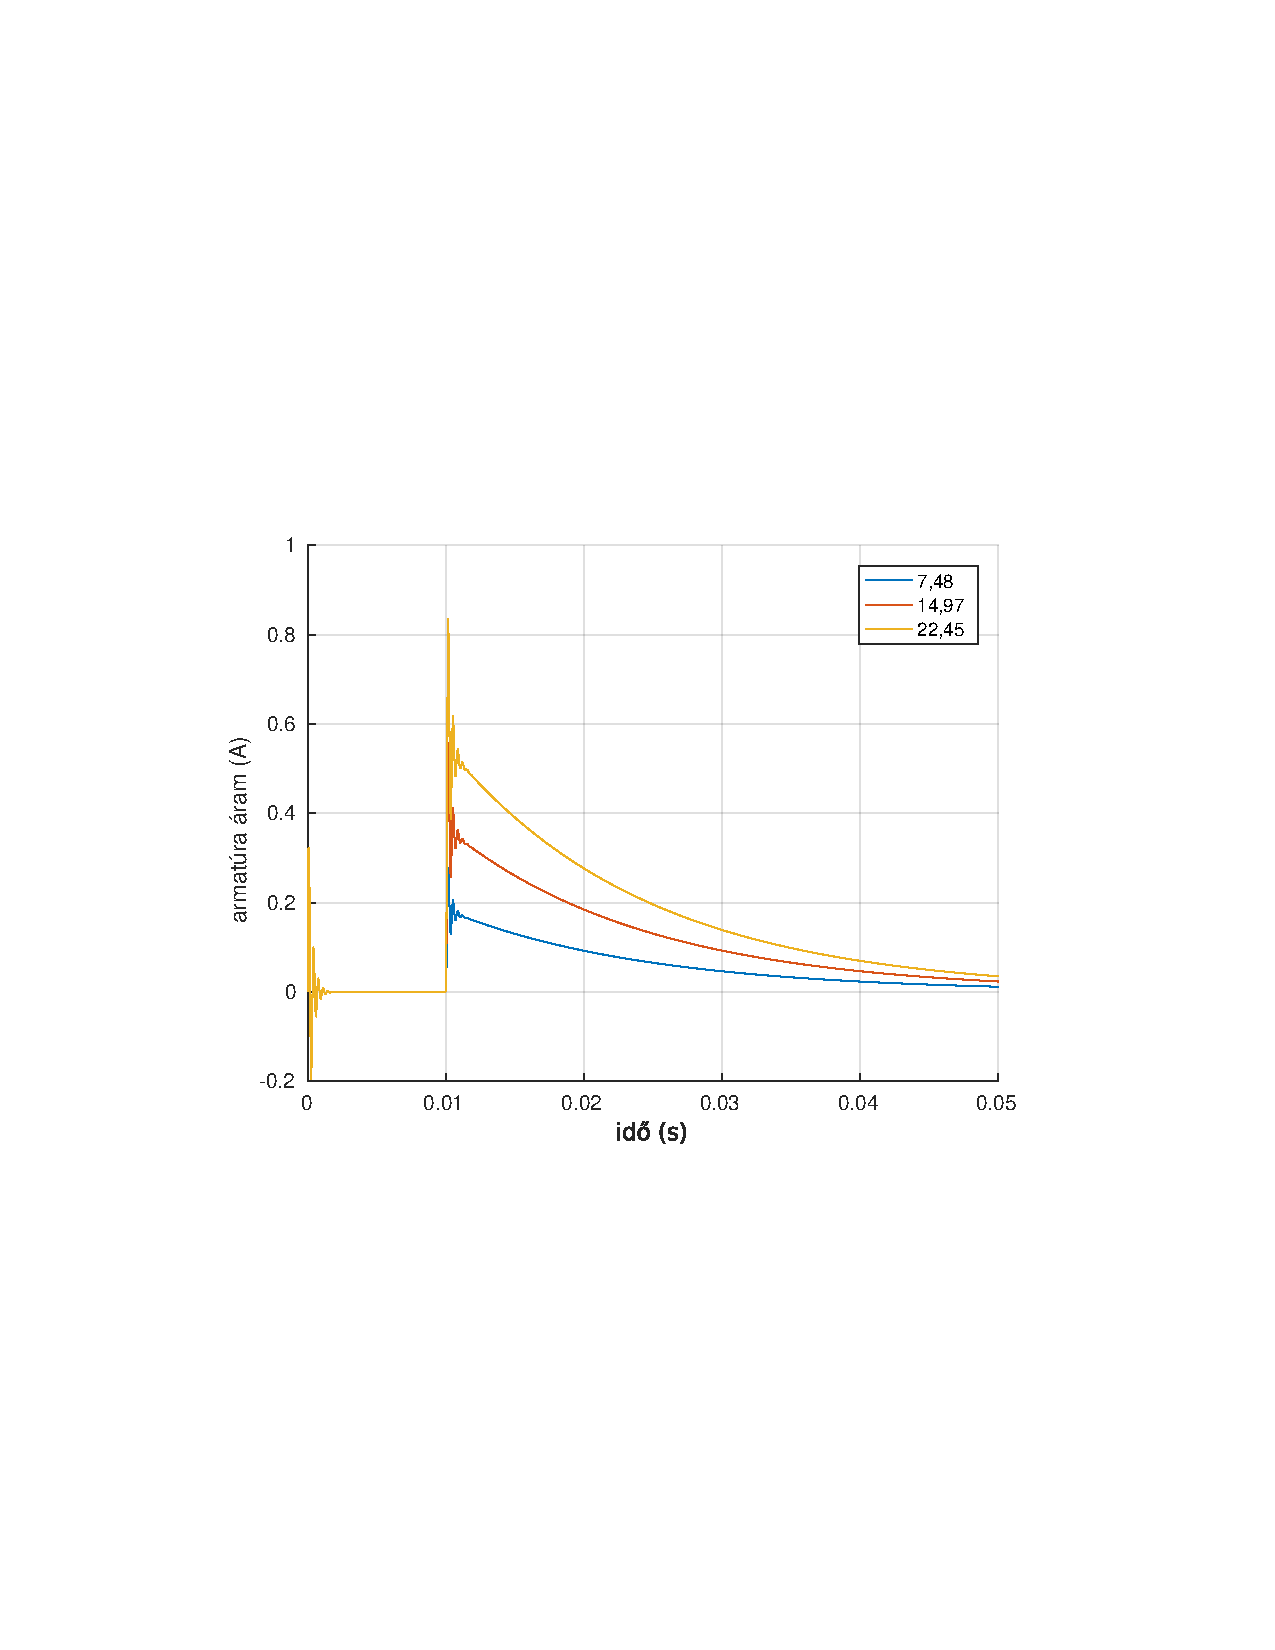
\includegraphics[width=\linewidth, trim=100 240 80 252, clip]{5-i}
		\caption{Áram válasz}
	\end{subfigure}
	\caption{Különböző amplitúdókra adott válasz}
	\label{fig:szorg1}
\end{figure}

A maximális terhelőnyomaték
\begin{equation}
	\tau_\text{t}^\text{max} = \pm0,337\text{ Nm}
\end{equation}

Bár az első tranziens közben az áram meghaladja a névleges áramot, az állandósult állapot
után kezdünk vizsgálni, feltettük hogy a kezdeti áramot túlélte a motor.
